\documentclass[a4paper,10pt]{article}

% ------------------------------------
% packages
\usepackage[a4paper,margin=1in,footnotesep=2.2\baselineskip]{geometry}
\usepackage{multicol}
\usepackage{xcolor}
\usepackage{framed}
\usepackage{emoji}
\usepackage[most]{tcolorbox}
\usepackage{fancyhdr}
\usepackage[tracking=true]{microtype}
\usepackage{ragged2e}
\usepackage{listings}
\usepackage{color}
\usepackage{pagecolor}
\usepackage{pdftexcmds}
\usepackage{geometry}
\usepackage{upgreek}
\usepackage{accents}
\usepackage{caption}
\usepackage{amssymb}
\captionsetup{
  font=small,
  labelfont=bf,
  tableposition=top
}
\captionsetup[figure]{name=\mono{Figure}}

% ------------------------------------
% checksum = SHA-1
\makeatletter
\ifx\pdf@filemdfivesum\undefined\def\pdf@filemdfivesum#{\mdfivesum file}\fi
\let\filesum\pdf@filemdfivesum
\makeatother

% ------------------------------------
% color definitions
\definecolor{armygreen}{rgb}{0.14, 0.71, 0.15}
\definecolor{darkgreen}{rgb}{0.08, 0.48, 0.18}
\definecolor{darkred}{rgb}{0.86, 0.153, 0.153}
\definecolor{azure}{rgb}{0.0, 0.5, 1.0}
\definecolor{bole}{rgb}{0.82, 0.57, 0.22}
\definecolor{dkgreen}{rgb}{0,0.6,0}
\definecolor{gray}{rgb}{0.5,0.5,0.5}
\definecolor{mauve}{rgb}{0.58,0,0.82}
\definecolor{light-gray}{gray}{0.95}
\definecolor{bg}{HTML}{fcfcfa}
\definecolor{bt}{HTML}{ffebe6}

% ------------------------------------
% code styling
\definecolor{shadecolor}{RGB}{180,180,180}
\newcommand{\code}[1]{\colorbox{shadecolor!30}{\mono{#1}}}
\newcommand{\zero}{{\raisebox{-0.7ex}{\LARGE\starg{o}}}}

% ------------------------------------
% digits
%\newcommand{\one}{{$\aleph$}}
%\newcommand{\two}{3}
%\newcommand{\three}{\uptheta}
%\newcommand{\four}{k}
%\newcommand{\five}{\raisebox{0.55ex}{\naskh{^^^^062d}}}
%\newcommand{\six}{{\hindi{^^^^096d}}}
%\newcommand{\seven}{\raisebox{0.3ex}{\robot{^^^^0434}}}
\newcommand{\one}{{\raisebox{-0.7ex}{\LARGE\starg{y}}}}
\newcommand{\two}{{\raisebox{-0.7ex}{\LARGE\starg{s}}}}
\newcommand{\three}{{\raisebox{-0.7ex}{\LARGE\starg{e}}}}
\newcommand{\four}{{\raisebox{-0.7ex}{\LARGE\starg{w}}}}
\newcommand{\five}{{\raisebox{-0.7ex}{\LARGE\starg{g}}}}
\newcommand{\six}{{\raisebox{-0.7ex}{\LARGE\starg{x}}}}
\newcommand{\seven}{{\raisebox{-0.7ex}{\LARGE\starg{t}}}}
\newcommand{\asserts}{\raisebox{0.10ex}{$\equiv$}}
\colorlet{Gray}{gray!20!}
\tcbset{on line, arc=1pt, leftrule=0.25pt,rightrule=0.25pt,toprule=0.25pt,bottomrule=0.25pt,
	boxsep=3pt, left=0pt,right=0pt,top=0pt,bottom=0pt,
	colframe=white,colback=Gray,  
	highlight math style={enhanced}
}
\lstdefinelanguage{Solidity}{
  %keywords={bool, true, false, return, address, bytes32, bytes4, bytes1, bytes, uint256, uint8, uint, string, if, while, else, case, break},
  keywords={},
  keywordstyle=\color{blue}\bfseries,
  %ndkeywords={function,struct, mapping, export, throw, implements, import, this},
  ndkeywords={},
  ndkeywordstyle=\color{darkgreen}\bfseries,
  identifierstyle=\color{black},
  sensitive=false,
  comment=[l]{//},
  morecomment=[s]{/*}{*/},
  commentstyle=\color{green}\mono,
  stringstyle=\color{orange}\mono,
  morestring=[b]',
  morestring=[b]",
  mathescape=true,
  literate={=>}{${\rightarrow}{}$}{1}
}
\lstset{
  backgroundcolor=\color{light-gray},
  language=Solidity,
  aboveskip=3mm,
  belowskip=3mm,
  showstringspaces=false,
  columns=flexible,
  basicstyle={\footnotesize\mono},
  numbers=none,
  numberstyle=\tiny\color{gray},
  keywordstyle=\color{blue},
  commentstyle=\color{dkgreen},
  stringstyle=\color{mauve},
  breaklines=true,
  breakatwhitespace=true,
  tabsize=3
}

% ------------------------------------
% fonts
\newfontfamily\pro[Path=./]{SFPro.ttf}
\newfontfamily\pbold[Path=./]{SFMonoSemiBold.ttf}
\newfontfamily\mono[Path=./]{SFMono.ttf}
\newfontfamily\mbold[Path=./]{SFMonoSemiBold.ttf}
\newfontfamily\hindi[Path=./]{Martel.ttf}
\newfontfamily\naskh[Path=./]{Naskh.ttf}
\newfontfamily\robot[Path=./]{Roboto.ttf}
\newfontfamily\victr[Path=./]{VictorMono.ttf}
\newfontfamily\starg[Path=./]{Stargate.ttf}

% ------------------------------------
% heading font-size
\usepackage{sectsty}
\usepackage{fontspec}
\sectionfont{\fontsize{12}{15}\selectfont}
\usepackage[utf8]{inputenc}

% ------------------------------------
% footnote positioning
\usepackage[hang,flushmargin,bottom]{footmisc} 

% ------------------------------------
% bibliography
\usepackage[colorlinks=true,
            linkcolor=blue,
            urlcolor=blue,
            citecolor=blue,
            pdfauthor={sshmatrix},
            pdftitle={Helix2 Protocol},
            pdfsubject={Link Service and Protocol},
            pdfkeywords={ethereum, account, abstraction, link, name, decentralised, distributed},
            pdfproducer={sshmatrix},
            pdfcreator={sshmatrix}]{hyperref}
            
% ------------------------------------
% blank footnote
\newcommand\blfootnote[1]{%
	\begingroup
	\renewcommand\thefootnote{}\footnote{#1}%
	\addtocounter{footnote}{-1}%
	\endgroup
}

% ------------------------------------
% header
\pagestyle{fancy}
\fancyhf{}
\lfoot{\footnotesize \mono{\#}\tcbox{\mono{\filesum{\jobname}}}}
\begin{document}
\setcounter{footnote}{0}
\newpage
\topskip15pt

\fancyhead[L]{\footnotesize \mono{author}:\tcbox{\mono{sshmatrix}}}
\fancyhead[R]{{\footnotesize \mono{\href{https://github.com/sshmatrix/research}{github.com/sshmatrix/research/ecTopology}}}}
\fancyhead[C]{{\footnotesize \emoji{dna}}}
\fancyfoot[C]{{\footnotesize \mono{\thepage}}}
\fancyfoot[R]{{\footnotesize \mono{\today} \emoji{dna}}}

\begin{center}
	\textbf{\Large\pbold{\textls[-40]{Topological Interpretation of Elliptic Curves}}}\\
	\vspace{0.075in}
	\textls[-50]{\mono{Topological Interpretation of Finite Cyclic Groups}}\linebreak\linebreak
	\vspace{-0.175in}
	\textls[0]{\mono{Avneet Singh}}\linebreak\linebreak
	\textls[0]{\mono{Interplanetary Company UG}}\linebreak
	\textls[0]{\mono{\href{mailto:sshmatrix@proton.me}{sshmatrix@proton.me}}}\linebreak
\end{center}
\begin{center}
	\textbf{\Large\pbold{ABSTRACT}}\linebreak\linebreak
	\textls[-50]{\mono{Elliptic curves form the backbone of most cryptography today and are expected to feature in the post-quantum world through Zero-Knowlege algorithms. Most literature on Elliptic curves starts from the definition of a cubic symmetric polynomial and builds upon the group theoretic interpretation of finite fields. This may be sufficient to grasp the mere necessary details for implementing Elliptic curves in practise, but not necessarily ideal if one wants to understand why Elliptic curve geometry is unique and useful. To most readers, it can appear that Elliptic curves were drawn from a magic hat. In paper will illustrate that this is clearly not the case and there exists a very legitimate reason for how and why the humanity ended up using Elliptic curves for cryptography.}}
\end{center}
\vspace{0.2in}
\begin{flushleft}
	\textbf{\Large\pbold{INTRODUCTION}}\linebreak\linebreak
	\textls[-50]{\mono{This paper is intended as a standalone appendix to the main paper titled 'Intuitive Interpretation of Non-Interactive Zero-Knowledge Cryptography' [1]. The main paper deals with pretty much the entire field of cryptography starting from basic RSA to advanced Zero-Knowledge algorithms. In interest of conciseness, several important aspects of Elliptic curves couldn't be discussed in detail in the main paper; this document is an attempt to address those shortcomings for the overtly inclined reader. We'll also touch some peripheral topics that have tied number theory and elliptic curves at the hip. Having said that, we'll follow the same theme as the main paper and avoid jargon like plague.\linebreak\linebreak\linebreak
	}}
	\textbf{\Large\pbold{TO ELLIPTIC CURVES}}\linebreak\linebreak
	\textls[-50]{\mono{The hint is in the name. Elliptic curves are related to ellipses and their discovery was 'accidental' so to speak; most of the initial work toward elliptic curves was done by Newton, Legendre, Fermat, Euler, Abel and Jacobi. In simple terms, an elliptic curve is a paramterisation of an ellipse's circumference or arc length and it easily derivable. To begin with, consider an ellipse described by  its semi-major and -minor axis lengths of {\upalpha} and {\upgamma} (=\;1), i.e. eccentricity e\textsuperscript{2} = 1 - {1/\upalpha}\textsuperscript{2}. Such an ellipse is described by: ${\text{(1 - e\textsuperscript{2})}}\,{\text{x\textsuperscript{2}}} + \text{y\textsuperscript{2} = 1}$. We can simplify it further by safely\textsuperscript{\textcolor{blue}{1}}\blfootnote{\textls[-50]{\mono{\textsuperscript{1}{such that the values of both e and k lie between 0 and 1, aka [0, 1]}}}} replacing the constant 1 - e\textsuperscript{2} with k\textsuperscript{2}, yielding $\text{y\textsuperscript{2} = 1 - {\text{k\textsuperscript{2}}}\,{\text{x\textsuperscript{2}}}}$. Let's try to calculate the circumference C(k) of this ellipse; this will equivalent to integrating ({\updelta}x\textsuperscript{2} + {\updelta}y\textsuperscript{2})\textsuperscript{1/2} along the curve in one of the four cartesian quarters and then multiplying it by 4. This results in
	\vspace{4mm}
	\begin{center}
	C(e) = 4\,{\Large\robot{^^^^2211}}\;({\updelta}x\textsuperscript{2} + {\updelta}y\textsuperscript{2})\textsuperscript{1/2}, for x = [0, {\upalpha}], 
	\end{center}
	\begin{flushright}
		{\vspace{-8mm}\mono{(1)}}
	\end{flushright}
	\vspace{2mm}
	\begin{center}
	C(e) = 4\,{{\Large\robot{^^^^2211}}\hspace{0.3mm}\textsuperscript{\textsuperscript{\scriptsize{\upalpha}}}}{\hspace{-2.0mm}\textsubscript{\textsubscript{\scriptsize{0}}}}\;({\updelta}x\textsuperscript{2} + {\updelta}y\textsuperscript{2})\textsuperscript{1/2} = 4\upalpha\,{{\Large\robot{^^^^2211}}\hspace{0.3mm}\textsuperscript{\textsuperscript{\scriptsize{1}}}}{\hspace{-1.8mm}\textsubscript{\textsubscript{\scriptsize{0}}}}\;\Big[$\displaystyle\frac{\text{1 - e\textsuperscript{2}x\textsuperscript{2}}}{\text{1 - x\textsuperscript{2}}}$\Big]\textsuperscript{\textsuperscript{\scriptsize{1/2}}}\,{\updelta}x.
	\end{center}
	\begin{flushright}
		{\vspace{-8mm}\mono{(2)}}
	\end{flushright}
	\vspace{2mm}
	This is already the {\mbold{elliptic integral}} of the second kind{\textsuperscript{\textcolor{blue}{2}}\blfootnote{\textls[-50]{\mono{\textsuperscript{2}{'second kind' due to the presence of {\uptheta} in the numerator in its parameterised form; 'first kind' has 1 in the numerator}}}}} and it is particularly difficult to evaluate analytically. When e = 1 (k = 0), it is straightforward and evaluates to 4$\text{\upalpha}$ as expected. When e = 0 (i.e. circles; k = 1), it is also relatively straightforward and evaluates naturally to
	\vspace{2mm}
	\begin{center}
	C(e)\textsubscript{k\,=\,1} = 4\upalpha\,{{\Large\robot{^^^^2211}}\hspace{0.3mm}\textsuperscript{\textsuperscript{\scriptsize{1}}}}{\hspace{-1.8mm}\textsubscript{\textsubscript{\scriptsize{0}}}}$\displaystyle\frac{\text{1}}{\text{(1 - x\textsuperscript{2})\textsuperscript{1/2}}}$\,{\updelta}x = 4\upalpha\,{{\Large\robot{^^^^2211}}\hspace{0.3mm}\textsuperscript{\textsuperscript{\scriptsize{1}}}}\hspace{-1.8mm}{\textsubscript{\textsubscript{\scriptsize{0}}}}\;sin\textsuperscript{-1}(x) = 2{\uppi}\upalpha.
	\end{center}
	\begin{flushright}
		{\vspace{-8mm}\mono{(2a)}}
	\end{flushright}
	\vspace{2mm}
	In conjunction with the well-known trigonometric parameterisation of ellipse with (x, y) {\rightarrow} ({\upalpha}\,sin{\,\uptheta}, {\upgamma\,}cos{\,\uptheta}), the general elliptic intergal reduces to,
	\vspace{2mm}
	\begin{center}
	C(e) = \,{{\Large\robot{^^^^2211}}\hspace{0.3mm}\textsuperscript{\textsuperscript{\scriptsize{\uppi/2}}}}{\hspace{-4.5mm}\textsubscript{\textsubscript{\scriptsize{0}}}}\;\;\;(1 - e\textsuperscript{2}sin\textsuperscript{2}{\uptheta})\textsuperscript{1/2}\,{\updelta}{\uptheta}.
	\end{center}
	\begin{flushright}
		{\vspace{-8mm}\mono{(3)}}
	\end{flushright}
	\vspace{2mm}
	In strict sense, the inverse of the integrand in the elliptic integral (2)-(3) is already the elliptic curve, but it is not straightforward to interpret in this form. In order to arrive at a more intuitive and interpretive form of elliptic curve, we perform a paramterisation of the form {\uptheta}\textsuperscript{n} = 1 - e\textsuperscript{2}x\textsuperscript{2}. Let's consider in particular the parametrisation for n = 1, such that {\uptheta} = 1 - e\textsuperscript{2}x\textsuperscript{2}. This leads to
	\vspace{2mm}
	\begin{center}
	C(k) = $\displaystyle\frac{\text{1}}{\text{2}}$\,{{\Large\robot{^^^^2211}}\textsuperscript{\textsuperscript{\scriptsize{1}}}}{\hspace{-1.8mm}\textsubscript{\textsubscript{\scriptsize{k}\textsuperscript{2}}}}\;\hspace{-1.5mm}$\displaystyle\frac{\text{{\uptheta}}}{\text{[\uptheta({\uptheta} - k\textsuperscript{2})({\uptheta} - 1)]}\textsuperscript{\textsuperscript{\scriptsize{1/2}}}}$\,{\updelta}{\uptheta} = $\displaystyle{-}\frac{\text{\mbold{i}}}{\text{2}}$\,{{\Large\robot{^^^^2211}}\textsuperscript{\textsuperscript{\scriptsize{1}}}}{\hspace{-1.8mm}\textsubscript{\textsubscript{\scriptsize{k}\textsuperscript{2}}}}\;\hspace{-1.5mm}$\displaystyle\frac{\text{{\uptheta}}}{\text{\,E(\uptheta)}}$\,{\updelta}{\uptheta},
	\end{center}
	\begin{flushright}
		{\vspace{-8mm}\mono{(4)}}
	\end{flushright}
	\vspace{2mm}
	where {\mbold{i}} is the usual complex unit, i.e. {\mbold{i}} = $\sqrt{\text{-1}}$. The 3-order polynomial term in the denominator is of the form
	\vspace{2mm}
	\begin{center}
	{E\textsuperscript{2}(\uptheta)} = {\uptheta}\textsuperscript{3} + r\cdot\,{\uptheta}\textsuperscript{2} + p\,\cdot\,{\uptheta} + q,
	\end{center} 
	}}
\end{flushleft}
\vspace{2mm}
\begin{multicols}{2}
	\noindent
	\textls[-50]{\mono{which is precisely the more recognisable form of the {\mbold{elliptic curve}}! Note that the form of {E({\uptheta})} in the above example asserts three roots of {E(\uptheta)}, i.e. 0, k\textsuperscript{2}, 1. This is however not true for generic elliptic curves which may have only one real root depending on the values of p, q and r, all of which are functions of k in return. In our particular example, r = -(1 + k\textsuperscript{2}), p = k\textsuperscript{2} and q = 0. Some readers may feel cheated at this point since we have just said that an elliptic curve is simply the square root of a cubic polynomial! This is indeed correct but not every cubic polynomial is an elliptic curve; the coefficients of the cubic polynomial must be such that there are no repeated roots, i.e. they represent a legitimate ellipse with legal values of e\textsuperscript{2} and k\textsuperscript{2}.
	}}
	\noindent
	\begin{minipage}{\linewidth}
		\centering
		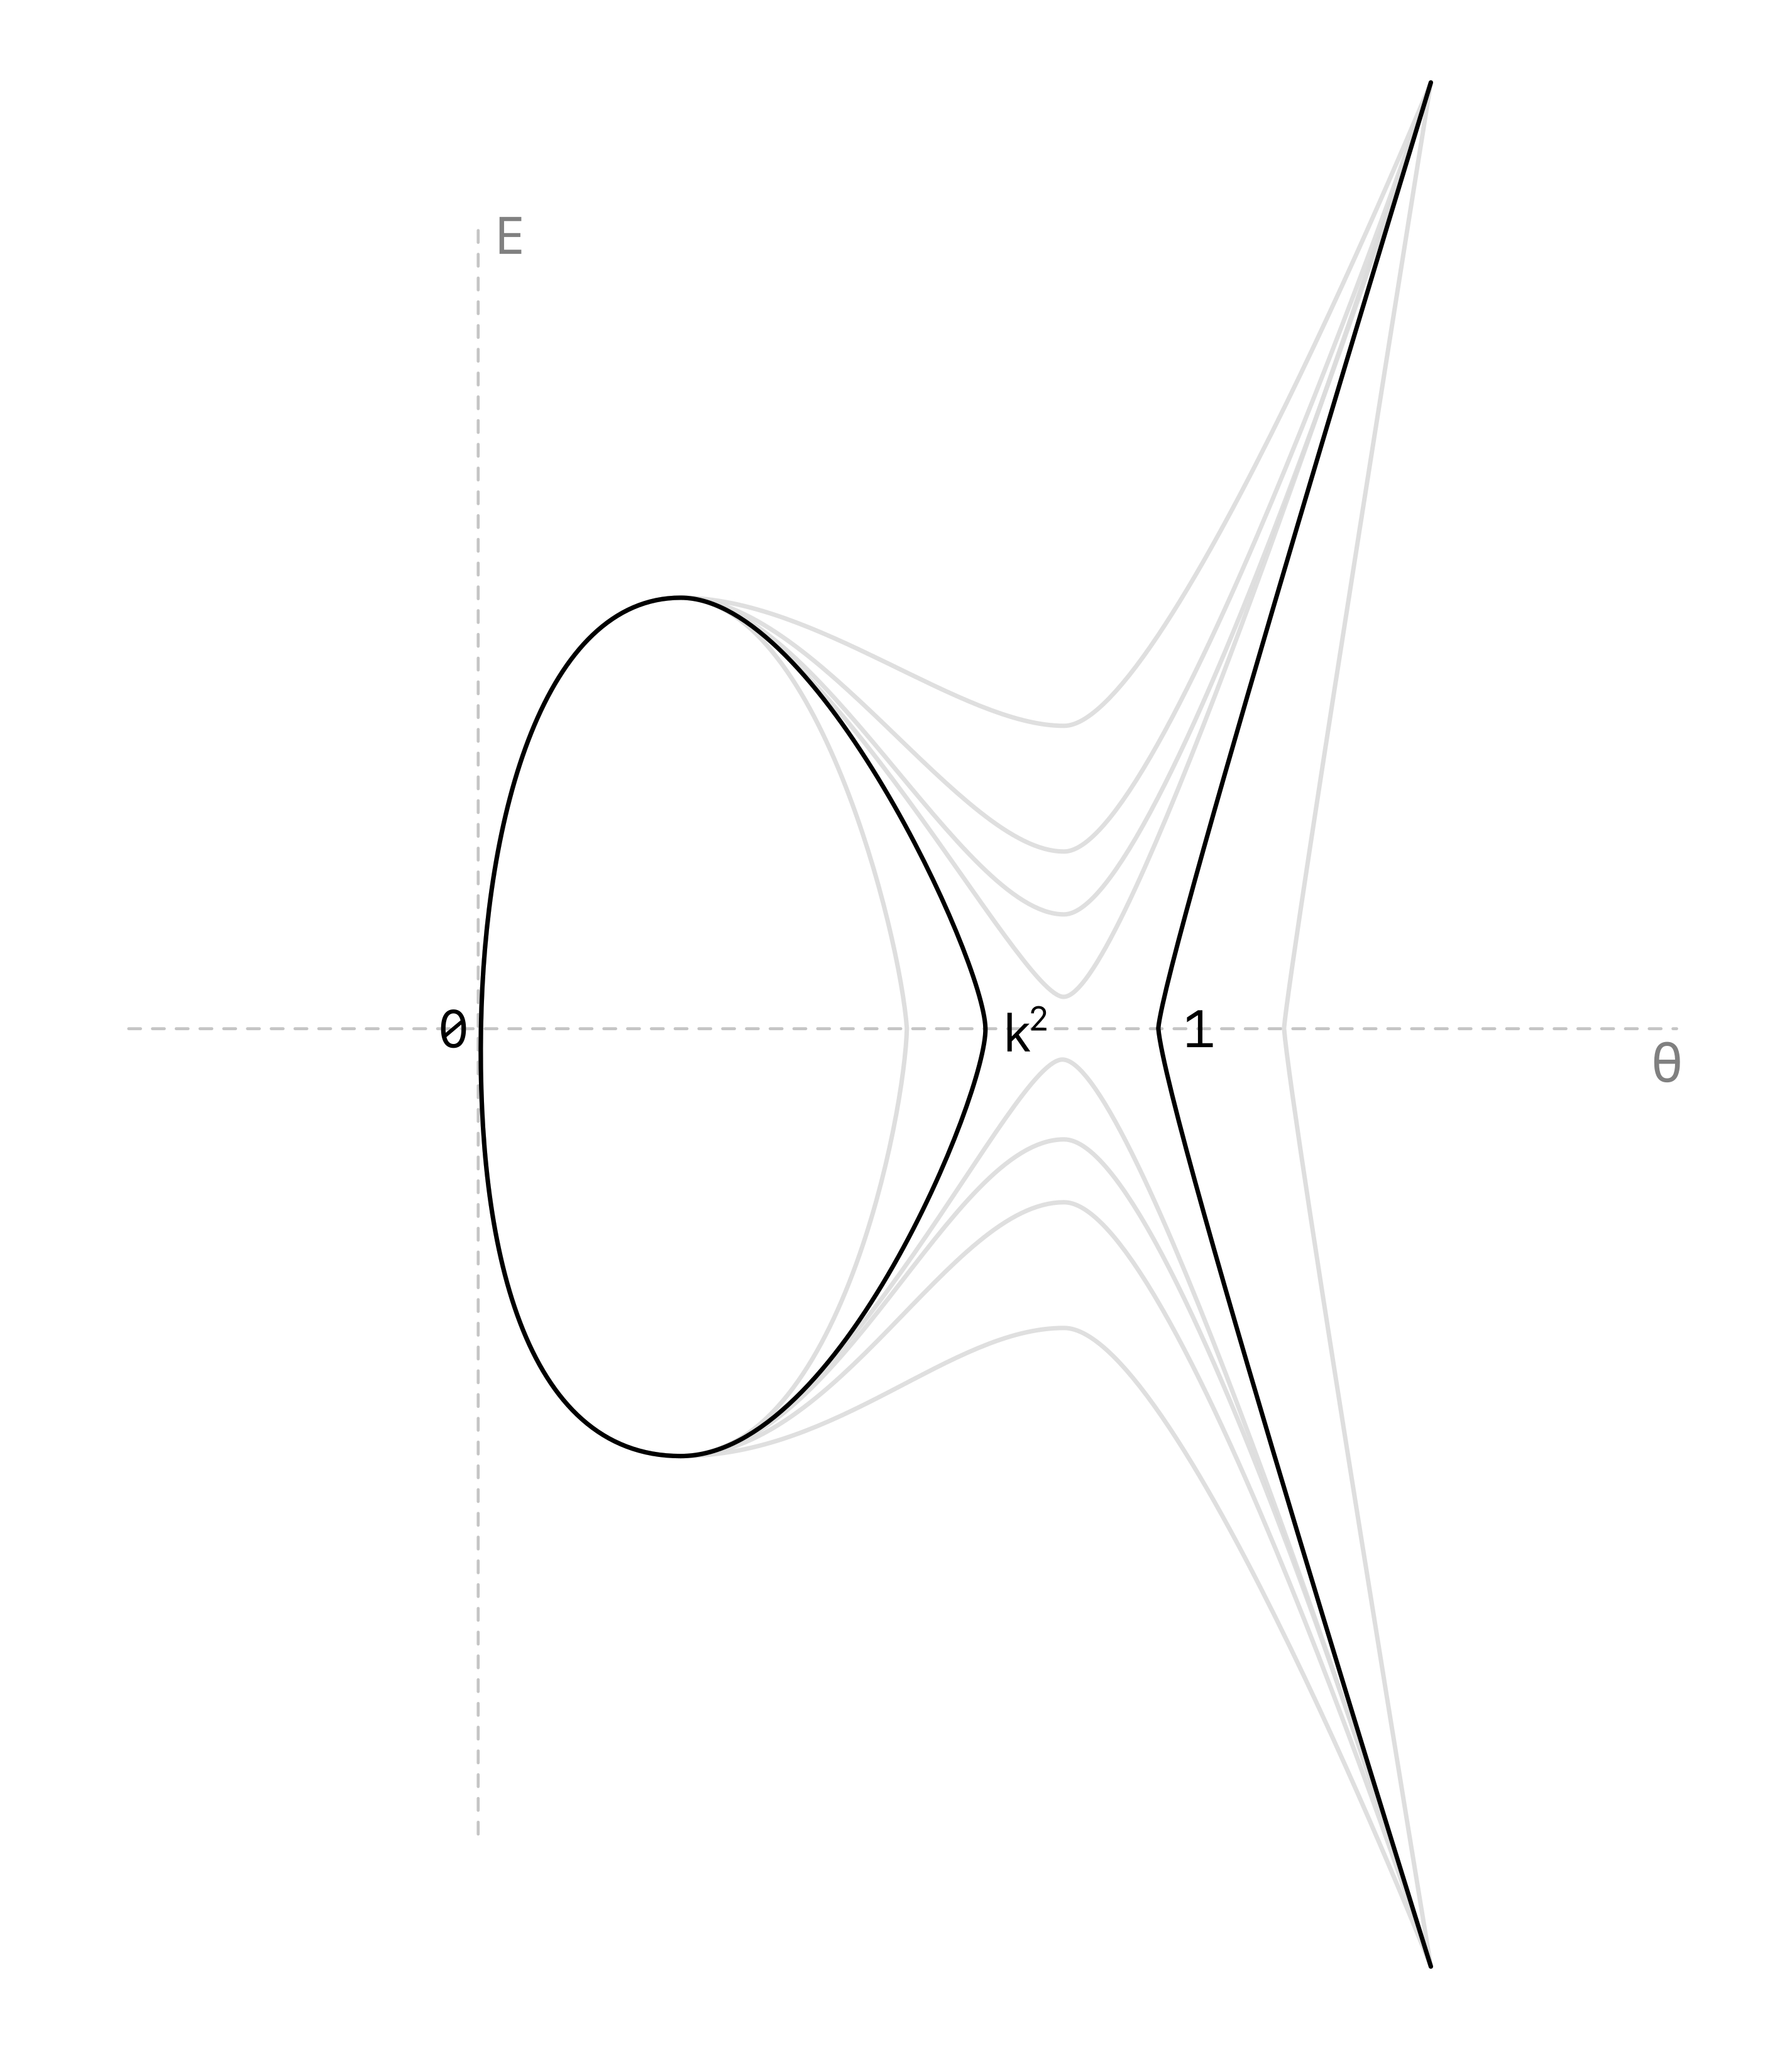
\includegraphics[width=60mm]{./img/ellipticCurve.png}\vspace{1mm}
		\captionof{figure}{\textls[-50]{\mono{Family of projected curves with one and three real root(s) in $\mathbb{R}$ space}}}
		\label{fig:ec}
	\end{minipage}
	\linebreak
\end{multicols}
\begin{flushleft}
	\textls[-50]{\mono{Lastly, we note that the if the elliptic curve has 3 real roots, then evaluation of (4) requires integrating {E(\uptheta)} in the range (k\textsuperscript{2}, 1) where it is purely complex! In other words, figure \ref{fig:ec} doesn't paint the entire picture of elliptic curves with three real roots instead of one. To fully grasp the topological intuition behind {E(\uptheta)}, we must include the complex plane in our graphics.
	\linebreak\linebreak\linebreak
	\textbf{\Large\pbold{\textls[0]{INITIATION BY JACOBI}}}\linebreak\linebreak
	It was Abel who first understood that the inverse of the intergal in (2a) is periodic and more relevant than the intergal itself, i.e.
	\vspace{2mm}
	\begin{center}
	F\textsuperscript{-1}($\bar{\text{x}}$) = 1\,/\,{{\Large\robot{^^^^2211}}\hspace{0.3mm}\textsuperscript{\textsuperscript{\scriptsize{$\bar{\text{x}}$}}}}{\hspace{-1.8mm}\textsubscript{\textsubscript{\scriptsize{0}}}}$\displaystyle\frac{\text{1}}{\text{(1 - x\textsuperscript{2})\textsuperscript{1/2}}}$\,{\updelta}x = sin\textsuperscript{-1\textsuperscript{\scriptsize{-1}}}($\bar{\text{x}}$) = sin($\bar{\text{x}}$),
	\end{center}
	\begin{flushright}
		{\vspace{-8mm}\mono{(5)}}
	\end{flushright}
	\vspace{2mm}
	Legendre in the past had re-arranged equation (2) in another form which turned out to be more useful for Jacobi. Legendre's form of (2) simply reads
	\begin{center}
	C(e) = 4\upalpha\,{{\Large\robot{^^^^2211}}\textsuperscript{\textsuperscript{\scriptsize{1}}}}{\hspace{-1.8mm}\textsubscript{\textsubscript{\scriptsize{0}}}}\;$\displaystyle\frac{\text{1 - e\textsuperscript{2}x\textsuperscript{2}}}{\text{[(1 - x\textsuperscript{2})(\text{1 - e\textsuperscript{2}x\textsuperscript{2}})]\textsuperscript{\textsuperscript{\scriptsize{1/2}}}}}$\,{\updelta}x,
	\end{center}
	\begin{flushright}
		{\vspace{-8mm}\mono{(6)}}
	\end{flushright}
	\vspace{2mm}
	Legendre noted that integrating the elliptic integral of second kind is easier if one knows the integral evaluation of the first kind{\textsuperscript{\textcolor{blue}{2}}\blfootnote{\textls[-50]{\mono{\textsuperscript{2}{one can observe this by integrating (6) using the elementary 'by parts' formalism}}}}}, i.e. the same equation as above but with the numerator set to 1,
	\begin{center}
	C($\bar{\text{x}}$) = 4\upalpha\,{{\Large\robot{^^^^2211}}\textsuperscript{\textsuperscript{\scriptsize{$\bar{\text{x}}$}}}}{\hspace{-1.8mm}\textsubscript{\textsubscript{\scriptsize{0}}}}\;$\displaystyle\frac{\text{1}}{\text{[(1 - x\textsuperscript{2})(\text{1 - e\textsuperscript{2}x\textsuperscript{2}})]\textsuperscript{\textsuperscript{\scriptsize{1/2}}}}}$\,{\updelta}x.
	\end{center}
	\begin{flushright}
		{\vspace{-8mm}\mono{(7)}}
	\end{flushright}
	\vspace{2mm}
	In parameterised form, elliptic integral of the first kind reads,
	\begin{center}
	C(e) = \,{{\Large\robot{^^^^2211}}\hspace{0.3mm}\textsuperscript{\textsuperscript{\scriptsize{\uppi/2}}}}{\hspace{-4.5mm}\textsubscript{\textsubscript{\scriptsize{0}}}}\;\;\;$\displaystyle\frac{\text{1}}{\text{(1 - e\textsuperscript{2}sin\textsuperscript{2}{\uptheta})\textsuperscript{1/2}}}$\,{\updelta}{\uptheta},
	\end{center}
	\begin{flushright}
		{\vspace{-8mm}\mono{(8)}}
	\end{flushright}
	\vspace{2mm}
	which is eerily innocent-looking and quite similar to (3) except that the integrand is inverted. This particular form of the elliptic integral of the first kind circle is where Jacobi made the first meaningful step toward parameterising generic elliptic curves. While generalising the integral F(x) to F(e,\,x) for non-zero e, Jacobi concluded that he didn't in fact need to solve the integral but instead simply attempt to gauge its properties (e.g. periodicity) by analysing the integrant. Jacobi's playtime revealed that the symmetric appearance of the terms e\textsuperscript{2} and x\textsuperscript{2} in the general elliptic integral equates to a bi-periodic function with complex periods! In simpler words, equation (7) is double-periodic with both periods ($\hat{\upomega}$\textsubscript{1},\,$\hat{\upomega}$\textsubscript{2}\;{$\in$}\;{$\mathbb{C}$}) being complex numbers, such that C($\bar{\text{x}}$) = C($\bar{\text{x}}$ + n\textsubscript{1}\,\cdot\,$\hat{\upomega}$\textsubscript{1}) = C($\bar{\text{x}}$ + n\textsubscript{2}\,\cdot\,$\hat{\upomega}$\textsubscript{2}), where $\hat{\upomega}$\textsubscript{1} and $\hat{\upomega}$\textsubscript{2} must necessarily be linearly-independent in {$\mathbb{R}$}, aka they are not mutually related by  $\hat{\upomega}$\textsubscript{1}\,{\robot{^^^^2260}}\;{$\mathbb{R}$}\,\cdot\,$\hat{\upomega}$\textsubscript{2}. Jacobi had arrived at this result after he fucked around with C($\bar{\text{x}}$) and assumed it to be a sine-inverse-like function{\textsuperscript{\textcolor{blue}{2}}\blfootnote{\textls[-50]{\mono{\textsuperscript{2}{due to the said integral being literally sin\textsuperscript{-1}($\bar{\text{x}}$) for e = 0}}}}} (denoted sin\textsuperscript{-1}\hspace{-3.0mm}\textsubscript{L}\hspace{1.3mm}$\bar{\text{x}}$), and found out that it did in fact have properties similar to a sinusoid such as periodicity. This however wasn't the most important assertion; Jacobi further found that no single-variable function could possibly have more than two independent complex periods, and all except elliptic integrals of the first and second (and third) kind have at most one period only! This was arguably the first solid proof that elliptic integrals were a special class of functions. What about the values of $\hat{\upomega}$\textsubscript{1} and $\hat{\upomega}$\textsubscript{2} though?\linebreak\linebreak\linebreak
	\textbf{\Large\pbold{\textls[0]{COMPLEX DOMAIN}}}\linebreak\linebreak
	We are now at a point where we cannot avoid complex numbers any further. We faced them while trying to evaluate the elliptic integral when {E($\uptheta$)} had three real roots. Now we are facing them yet again when trying to retrace Jacobi's steps. Eisenstein was first to truly accept that it is perhaps better to begin the description of elliptic integrals in the complex space and then project the findings in the real space, instead of trying to analyse it all in real space alone. We will get there in the next section but we must first introduce complex numbers and particularly n-dimensional lattices in complex space, both of which are necessary to understand bi-periodic functions with complex periods.
	\linebreak\linebreak\linebreak
	}}
	\textbf{\Large\pbold{\textls[0]{EISENSTEIN'S ENGINEERING}}}\linebreak\linebreak
	\textls[-50]{\mono{-
	}}
\end{flushleft}
\begin{flushleft}
	\textbf{\Large\pbold{REFERENCES}}\linebreak\linebreak
		\textls[-50]{\mono{
			[1] Intuitive Interpretation of Non-Interactive Zero-Knowledge Cryptography\linebreak
		}}
\end{flushleft}
\begin{flushright}
	\textbf{\large\pbold{METADATA}}\linebreak\linebreak
	\textls[-50]{\mono{
		\mono{Github: }\tcbox{}\linebreak
		\mono{Contracts: }\tcbox{}\linebreak
		\mono{Source: }\tcbox{}\linebreak
		\mono{SHA-1 Checksum: }\tcbox{}\linebreak
		\mono{Date: }\tcbox{\mono{\today}}\linebreak
	}}
\end{flushright}
\end{document}
